\documentclass[12pt,oneside]{fithesis2}


\usepackage[english]{babel}
\usepackage[utf8]{inputenc}
\usepackage{lmodern}
\usepackage[T1]{fontenc}

\usepackage[scaled=0.86]{berasans}
\usepackage[scaled=1.03]{inconsolata}
\usepackage[plainpages=false, pdfpagelabels]{hyperref}

\usepackage{enumitem}
\usepackage{microtype}
\usepackage[top=3.0cm, bottom=3.5cm, left=2.4cm, right=2.4cm]{geometry}	% pc version
%\usepackage[top=3.0cm, bottom=3.5cm, left=2.9cm, right=1.9cm]{geometry}	% print version

\usepackage[backend=biber,style=ieee]{biblatex}
\addbibresource{thesis.bib}

\usepackage{minted}
\setminted{framesep=2mm, frame=lines}

\usepackage{multicol}

\usepackage{tikz}
\usetikzlibrary{trees,calc,shapes.arrows}


\thesislang{en}
\thesistitle{GPU-based speedup of EACirc project}
\thesissubtitle{Bachelor Thesis}
\thesisstudent{Jiří Novotný}
\thesiswoman{false}
\thesisfaculty{fi}
\thesisyear{Spring 2015}
\thesisadvisor{RNDr. Petr Švenda, Ph.D.}



\newcommand{\todo}{
	%\bigskip
	\noindent
	{\large\color{red}\textbf{TODO}}
	%\bigskip
}



\begin{document}
\FrontMatter
	\ThesisTitlePage
	%\begin{ThesisDeclaration}
	%	\DeclarationText
	%	\AdvisorName
	%\end{ThesisDeclaration}
	%\begin{ThesisThanks}
		%TODO Thesis Thanks
	%\end{ThesisThanks}
	%\begin{ThesisAbstract}
		%TODO Thesis Abstract
	%\end{ThesisAbstract}
	%\begin{ThesisKeyWords}
		%TODO Thesis Keywords
	%\end{ThesisKeyWords}
	\tableofcontents

\MainMatter
\chapter{CMake}
The EACirc mainly consists of \emph{C} and \emph{C++} code. The code was divided into reasonably logical sections but the overall structure and concept of the project was monolithic.\footnote{A monolithic binary is an executable that does not need any other dependencies or resources at a runtime. In other words, the binary is independent.} This tended to compile all sources into one big executable approximately 9~MB in size which took some non-trivial time and also this design was not apt to scale.

On top of that EACirc is developed as a cross-platform application. To provide native builds for each supported platform (Windows \cite{win} and Linux) there was a special makefile, or an IDE specific project file, which described how to build the application. When a change in the build was introduced, e.g. a new source file was added, the change must have been manually propagated to all makefiles to provide consistency. This workflow was not easy to maintain and the violation of these rules could cause an uncomfortable pitfall.

To solve these problems the CMake \cite{cmake} tool was integrated into the project of EACirc. The tool is developed and maintained by Kitware, Inc. \cite{kitware} as an open-source software. The main purpose of this tool is to provide native builds of cross-platform applications and tries to minimize the effort to maintain the project.

Although there are many similar tools as CMake, and some of them provides better features, they are not so widely supported. CMake provides generation of project files for almost every common IDE and some of those IDEs comes with a support for CMake.

\section{CMake toolset}

The CMake is actually a set of several executables; the main executable \texttt{cmake} and the supportive ones \texttt{ccmake} (or \texttt{cmake-gui}), \texttt{ctest}, and \texttt{cpack}.

The \texttt{cmake} executable takes a configuration file called \texttt{CMakeLists.txt} distributed with the sources and generates the platform specific makefiles as an output. Then the user invokes a platform specific tool for building -- usually \texttt{make}, \texttt{ninja}, or \texttt{MSBuild}. If the process was successful the native binaries of the project are now made.

The \texttt{ctest} executable provides a simple platform for project testing. After the binaries are successfully build the invocation of \texttt{ctest} usually runs some user-defined test on top of them.

The last but not least executable \texttt{cpack} provides a cross-platform way to deploy your application on the target system.

The remaining executables \texttt{ccmake} and \texttt{cmake-gui} are just a more convenient ways to use a \texttt{cmake} executable since \texttt{cmake} has only a command line interface. The former provides a TUI\footnote{Text-based user interface (TUI)} and the latter provides GUI\footnote{Graphical user interface (GUI)}.

\section{A closer look to the \texttt{cmake} executable}

The \texttt{cmake} executable is not just a dummy build-system. The process of generating a makefile is far more complex. Firstly the user chooses the \emph{source directory} and the \emph{build directory}. Then he invokes the \texttt{cmake} command in a \emph{build directory} with appropriate parameters. The subsequent process consists of several phases -- selection of a native build-system (in a CMake terminology referenced as a \emph{generator}), configuration based on a user-specific input, and the own generation of a makefile.\footnote{Note that the exact scheme of this process can differ according to which interface of CMake is being used -- i.e. \texttt{cmake}, \texttt{ccmake}, or \texttt{cmake-gui}.}

The \emph{source directory} is simply a directory where the project sources are located and where the top-level \texttt{CMakeLists.txt} file is located, which is distributed with the sources. The build directory is an empty user-created directory where he wants the binaries to be build.

The selection of the \emph{generator} depends on the user's platform, on the user-installed native build-systems, and on the user's intentions. On Linux the generator used is usually \texttt{make} or \texttt{ninja}. When the user wants to generate a project files to a specific IDE, he chooses the appropriate generator -- e.g. Visual Studio 2013 \cite{msvc} on Microsoft Windows \cite{win}. Usually the selection of appropriate generator is done by CMake automatically.

The subsequent phase, configuration, is in place. Here the user specifies variable options for the build that the project supports. For instance some features of the application can be switched on/off or the location of a third party dependencies can be specified. Also the different build configuration can be switched, i.e. release or debug.

If the configuration is all right then the makefile is successfully created in the \emph{build directory}. Then we just invoke the appropriate tool to execute the makefile and the binaries are build.

There is a worth mentioning that the makefile automatically detects any changes made in the \emph{source directory} so the user invokes the \texttt{cmake} executable just once to generate the makefile or when he wants to change the variable options of the build. The makefile also provides a target for installing the application and/or a target fo testing.

The minimal and the most common sequence of commands to build and install a project on Linux using the CMake are:
	\begin{minted}[autogobble]{text}
	mkdir <build_directory>
	cd <build_directory>
	cmake <path_to_source_directory>
	make
	make install
	\end{minted}
Note that the \texttt{make} is chosen as a default generator and the default project settings and configurations are applied. The binaries are installed to the platform specific location, i.e. for Linux it is \texttt{/usr/share/local}.

\section{Changes made to the EACirc repository structure}

There had been made several changes to the EACirc repository structure. The new folder design should reflect the logical structure of the EACirc philosophy.

	\begin{figure}[H]
	\centering
	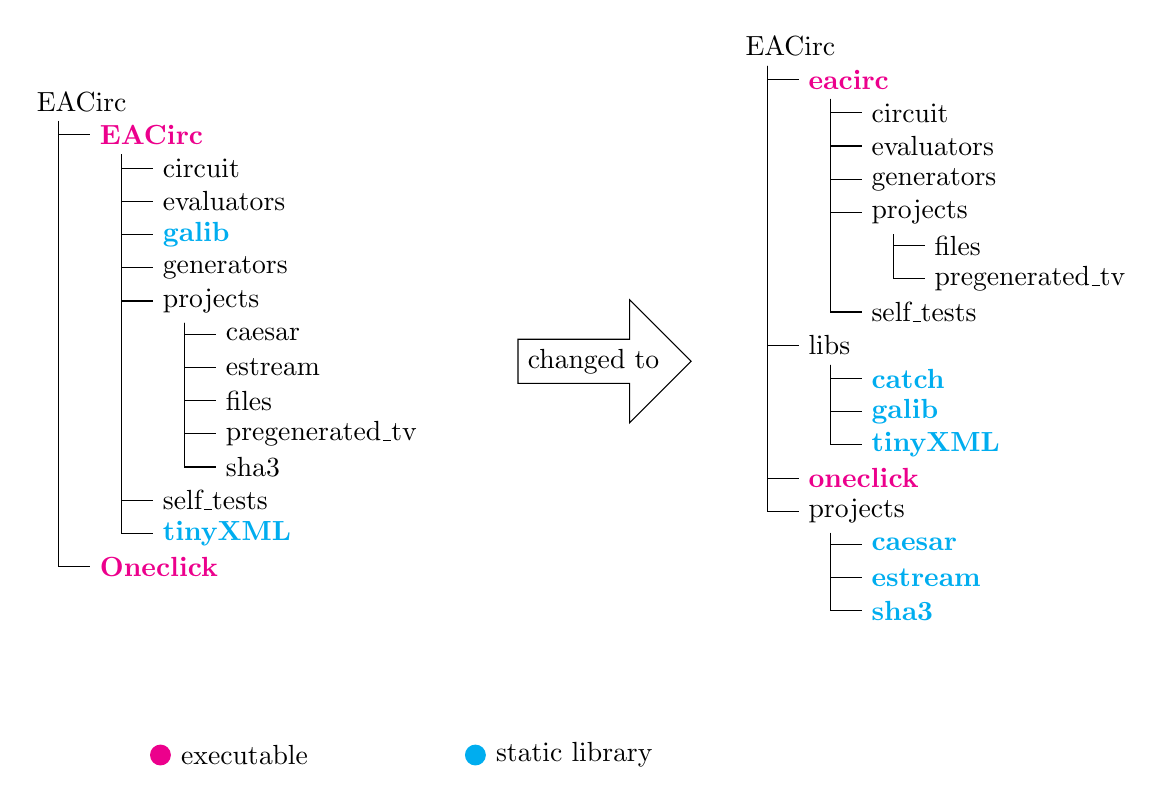
\begin{tikzpicture}[
grow via three points={one child at (0.8,-1.2em) and two children at (0.8,-1.2em) and (0.8,-2.4em)},
edge from parent path={($(\tikzparentnode\tikzparentanchor)+(.4cm,0pt)$) |- (\tikzchildnode\tikzchildanchor)},
growth parent anchor=west,
parent anchor=south west,
every child node/.style={anchor=west}
]
\node at (0,-2em) {EACirc}
	child { node [font=\bf,text=magenta] {EACirc}
		child { node {circuit} }
		child { node {evaluators} }
		child { node [font=\bf,text=cyan] {galib} }
		child { node {generators} }
		child { node {projects}
			child { node {caesar} }
			child { node {estream} }
			child { node {files} }
			child { node {pregenerated\_tv} }
			child { node {sha3} }
		}
		child [missing] {}
		child [missing] {}
		child [missing] {}
		child [missing] {}
		child [missing] {}
		child { node {self\_tests} }
		child { node [font=\bf,text=cyan] {tinyXML} }
	}
	child [missing] {}
	child [missing] {}
	child [missing] {}
	child [missing] {}
	child [missing] {}
	child [missing] {}
	child [missing] {}
	child [missing] {}
	child [missing] {}
	child [missing] {}
	child [missing] {}
	child [missing] {}
	child { node [font=\bf,text=magenta] {Oneclick}
	};
	
\node at (6.5, -4) [single arrow, draw, single arrow head extend=.5cm] {changed to};
		
\node at (9, 0) {EACirc}
	child { node [font=\bf,text=magenta] {eacirc}
		child { node {circuit} }
		child { node {evaluators} }
		child { node {generators} }
		child { node {projects}
			child { node {files} }
			child { node {pregenerated\_tv} }
		}
		child [missing] {}
		child [missing] {}
		child { node {self\_tests} }
	}
	child [missing] {}
	child [missing] {}
	child [missing] {}
	child [missing] {}
	child [missing] {}
	child [missing] {}
	child [missing] {}
	child { node {libs}
		child { node [font=\bf,text=cyan] {catch} }
		child { node [font=\bf,text=cyan] {galib} }
		child { node [font=\bf,text=cyan] {tinyXML} }
	}
	child [missing] {}
	child [missing] {}
	child [missing] {}
	child { node [font=\bf,text=magenta] {oneclick} }
	child { node {projects}
		child { node [font=\bf,text=cyan] {caesar} }
		child { node [font=\bf,text=cyan] {estream} }
		child { node [font=\bf,text=cyan] {sha3} }
	};
	
	\node at (1,-9) [scale=0.8,shape=circle,fill=magenta,label=right:executable] {};
	\node at (5,-9) [scale=0.8,shape=circle,fill=cyan,label=right:static library] {};
\end{tikzpicture}
	\caption{Old vs. new repository structure}
	\end{figure}
	
\noindent
The first and also the smallest change was to name all source folders with only small letters. Next the libraries from 3rd party providers, \texttt{catch}, \texttt{galib}, and \texttt{tinyXML}, were moved into the separate folder -- the \emph{libs} directory.

Then there was a request to isolate the so called \emph{projects}. A \emph{project} in EACirc terminology means a module for some problem solving. These \emph{projects} are \texttt{caesar}, \texttt{estream}, \texttt{sha3}, \texttt{files} and \texttt{pregenerated\_tv}. Since \texttt{files} and \texttt{pregenerated\_tv} are both just small modules consisting from only one source file, it would be impractical to isolated them. On the other hand the big modules \texttt{caesar}, \texttt{estream}, and \texttt{sha3} were moved to the the separate folder, called the \emph{projects} folder. Each of the isolated projects was made to compile into a static library.\footnote{There is a plan to remade the projects to modules loaded dynamically at runtime. This would require to compile them separately into the dynamic libraries.}

From the folders \texttt{eacirc} and \texttt{oneclick} are build executables named accordingly to their corresponding folders. The \emph{projects}, which are now compiled into the static libraries, are now statically linked to the \texttt{eacirc} executable, which represents the EACirc tool as a whole. The \texttt{oneclick} executable is a supportive tool for automated task management developed by Ľubomír Obrátil. \cite{oneclick}

\section{The new build-system of EACirc}

The new build-system is written on the CMake platform. This platform allows to define custom options for generating the build. Here is a descriptive list of EACirc specific options:

\begin{description}
	\item[\texttt{BUILD\_ONECLICK}]
	Enable building of Oneclick, the supportive tool for EACirc.
	
	\item[\texttt{BUILD\_CAESAR}]
	Enable building of the Caesar project.
	
	\item[\texttt{BUILD\_ESTREAM}]
	Enable building of the Estream project.
	
	\item[\texttt{BUILD\_SHA3}]
	Enable building of the SHA-3 project.
	
	\item[\texttt{BUID\_CUDA}]
	When enabled, EACirc is build to support CUDA devices. This option is available only if the CUDA Toolkit \cite{cuda_toolkit} is installed on the build machine\footnote{A build machine is a physical or a virtual machine that is used to build the project.} and found by the CMake.
\end{description}

\noindent
Since the \emph{projects} are build into static libraries they must be linked to the \texttt{eacirc} executable at the compile time. This is done automatically when the option for the specific \emph{project} is enabled. In the figure \ref{fig:deps} are shown the dependencies of the all build targets.
	\begin{figure}[H]
	\centering
	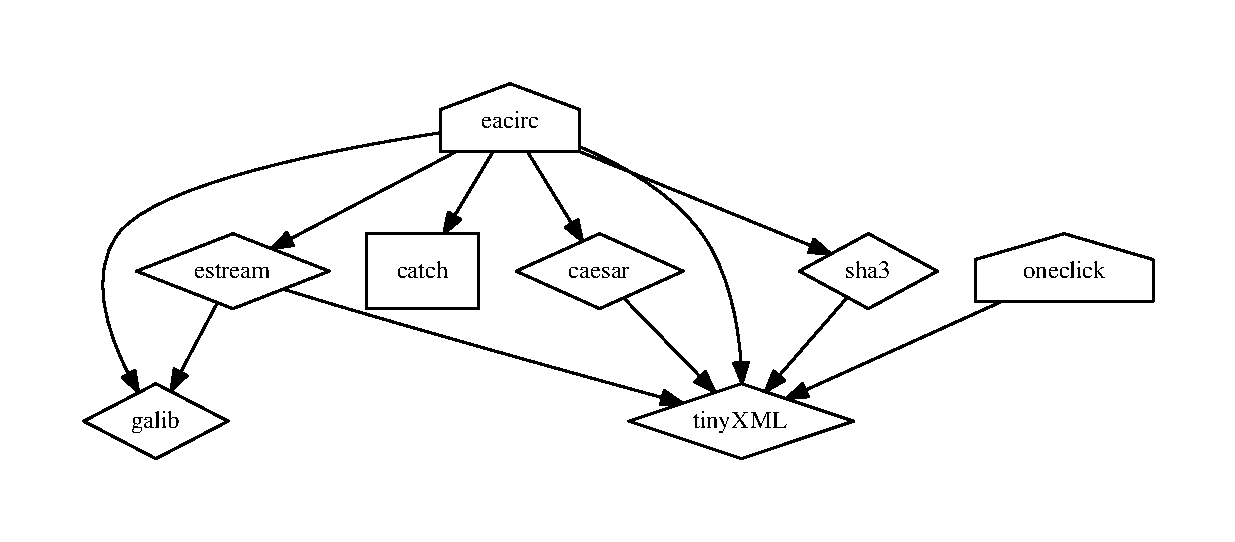
\includegraphics[width=.8\textwidth]{figures/deps}
	\caption{EAcirc dependency graph}
	\label{fig:deps}
	\small
	The static libraries are shown in the rhombus. The executables have a house around them. The square represents an interface library.\footnote{Interface library does not need to be linked against. It consists only of header files.} The direction of the arrows represents that some build target depends on another.
	\end{figure}

\noindent
The build-system is also version aware. The current version is stored in the \texttt{eacirc/Version.h} header file. The version corresponds to git commit hash \cite{git_book}. That means that for correct build generation there must be a git tools properly installed on the build machine and found by CMake.\footnote{If git tools are installed and not found automatically by CMake then the path to git tools can be specified manually.}

The usage of CMake and the new options of building EACirc are explained closely at the project Wiki page on Github under the Building EACirc section.

\section{Project settings for CUDA}

To set the project for CUDA is now much more easier with CMake support. When the CUDA Toolkit \cite{cuda_toolkit} is installed and automatically found by CMake\footnote{If CUDA Toolkit is installed on the build machine but not found by CMake automatically then the path to CUDA Toolkit can be specified manually.} then the option \texttt{BUILD\_CUDA} becomes available. If this option is enabled then the \texttt{eacirc} executable is build using Nvidia \cite{nvidia} \texttt{nvcc} compiler and the C preprocessor macro \texttt{CUDA} is defined causing that the executable will be runnable on CUDA capable devices. When writing a code for CUDA the preprocessor macro \texttt{CUDA} can be queried.

\printbibliography[heading=bibintoc]
\todo{Fix the autors of online resources}

\todo{Fix the titles in the bibliography to dislay big letters correctly.}

\todo{Cite Lobo's theses about oneclick and fix the source.}

\todo{Cite Martin Ukrop thesis in Introduction. What is EACirc?}

\end{document}